% !TEX TS-program = XeLaTeX
% use the following command:
% all document files must be coded in UTF-8
\documentclass[portuguese]{textolivre}
% build HTML with: make4ht -e build.lua -c textolivre.cfg -x -u article "fn-in,svg,pic-align"
\usepackage{polyglossia}
\setotherlanguage{english}
\setotherlanguage{chinese}
\newfontfamily\chinesefont{Noto Serif CJK SC}
\newfontfamily\cjkfont{Noto Serif CJK SC}
\newfontfamily\cjkfontsf{Noto Sans CJK SC}


\journalname{Texto Livre}
\thevolume{19}
%\thenumber{1} % old template
\theyear{2026}
\receiveddate{\DTMdisplaydate{2025}{11}{20}{-1}} % YYYY MM DD
\accepteddate{\DTMdisplaydate{2026}{3}{16}{-1}}
\publisheddate{\DTMdisplaydate{2026}{5}{21}{-1}}
\corrauthor{Júlio Reis Jatobá}
\articledoi{10.1590/1983-3652.2026.62945}
%\articleid{NNNN} % if the article ID is not the last 5 numbers of its DOI, provide it using \articleid{} commmand 
% list of available sesscions in the journal: articles, dossier, reports, essays, reviews, interviews, editorial
\articlesessionname{dossier}
\runningauthor{Jatobá} 
%\editorname{Leonardo Araújo} % old template
\sectioneditorname{Francis Arthuso Paiva~\orcid{0000-0002-9083-3342}}
\layouteditorname{Leonardo Araújo~\orcid{0000-0003-3884-2177}}


\title{Educação linguística em tempos de IA: multilinguismo, humanismo e formação de professores}
\othertitle{Language education in AI times: multilingualism, humanism, and teacher education}
% if there is a third language title, add here:
%\othertitle{Artikelvorlage zur Einreichung beim Texto Livre Journal}

\author[1]{Júlio Reis Jatobá~\orcid{0000-0001-5669-8119}\thanks{Email: \href{mailto:juliojatoba@um.edu.mo}{juliojatoba@um.edu.mo}}}
\affil[1]{University of Macau, Faculty of Arts and Humanities, Macau, China.}


\addbibresource{article.bib}

% use biber instead of bibtex
% $ biber article

% used to create dummy text for the template file
\definecolor{dark-gray}{gray}{0.35} % color used to display dummy texts
\usepackage{lipsum}
\SetLipsumParListSurrounders{\colorlet{oldcolor}{.}\color{dark-gray}}{\color{oldcolor}}

% used here only to provide the XeLaTeX and BibTeX logos
\usepackage{hologo}

% if you use multirows in a table, include the multirow package
\usepackage{multirow}

% provides sidewaysfigure environment
\usepackage{rotating}

% CUSTOM EPIGRAPH - BEGIN 
%%% https://tex.stackexchange.com/questions/193178/specific-epigraph-style
\usepackage{epigraph}
\renewcommand\textflush{flushright}
\makeatletter
\newlength\epitextskip
\pretocmd{\@epitext}{\em}{}{}
\apptocmd{\@epitext}{\em}{}{}
\patchcmd{\epigraph}{\@epitext{#1}\\}{\@epitext{#1}\\[\epitextskip]}{}{}
\makeatother
\setlength\epigraphrule{0pt}
\setlength\epitextskip{0.5ex}
\setlength\epigraphwidth{.7\textwidth}
% CUSTOM EPIGRAPH - END

% LANGUAGE - BEGIN
% ARABIC
% for languages that use special fonts, you must provide the typeface that will be used
% \setotherlanguage{arabic}
% \newfontfamily\arabicfont[Script=Arabic]{Amiri}
% \newfontfamily\arabicfontsf[Script=Arabic]{Amiri}
% \newfontfamily\arabicfonttt[Script=Arabic]{Amiri}
%
% in the article, to add arabic text use: \textlang{arabic}{ ... }
%
% RUSSIAN
% for russian text we also need to define fonts with support for Cyrillic script
% \usepackage{fontspec}
% \setotherlanguage{russian}
% \newfontfamily\cyrillicfont{Times New Roman}
% \newfontfamily\cyrillicfontsf{Times New Roman}[Script=Cyrillic]
% \newfontfamily\cyrillicfonttt{Times New Roman}[Script=Cyrillic]
%
% in the text use \begin{russian} ... \end{russian}
% LANGUAGE - END

% EMOJIS - BEGIN
% to use emoticons in your manuscript
% https://stackoverflow.com/questions/190145/how-to-insert-emoticons-in-latex/57076064
% using font Symbola, which has full support
% the font may be downloaded at:
% https://dn-works.com/ufas/
% add to preamble:
% \newfontfamily\Symbola{Symbola}
% in the text use:
% {\Symbola }
% EMOJIS - END

% LABEL REFERENCE TO DESCRIPTIVE LIST - BEGIN
% reference itens in a descriptive list using their labels instead of numbers
% insert the code below in the preambule:
%\makeatletter
%\let\orgdescriptionlabel\descriptionlabel
%\renewcommand*{\descriptionlabel}[1]{%
%  \let\orglabel\label
%  \let\label\@gobble
%  \phantomsection
%  \edef\@currentlabel{#1\unskip}%
%  \let\label\orglabel
%  \orgdescriptionlabel{#1}%
%}
%\makeatother
%
% in your document, use as illustraded here:
%\begin{description}
%  \item[first\label{itm1}] this is only an example;
%  % ...  add more items
%\end{description}
% LABEL REFERENCE TO DESCRIPTIVE LIST - END


% add line numbers for submission
%\usepackage{lineno}
%\linenumbers

\begin{document}
\maketitle

\begin{polyabstract}
\begin{abstract}
Este artigo examina, por meio de um estudo de caso qualitativo, como a Inteligência Artificial (IA) é integrada ao ensino de Português como Língua Estrangeira em Macau e quais implicações formativas e avaliativas essa integração produz. O objetivo é compreender os efeitos pedagógicos, políticos e éticos dessa incorporação, articulando multilinguismo, humanismo digital e formação docente. O \textit{corpus} reúne documentos institucionais, entrevistas e relatos de professores, além de produções discentes e registros de \textit{feedback} humano e automatizado, gerados entre 2023 e 2025 em duas disciplinas de graduação. À luz das literacias em IA e do conceito de \textit{interligências}, a análise identifica três padrões de uso da IA – assistivo, orientado e substitutivo – e evidencia tensões entre fluência textual, autoria, avaliação e mediação docente. Nos contextos investigados, a IA amplia as possibilidades de revisão e personalização, mas pode intensificar a dependência tecnológica e reduzir a visibilidade do processo de escrita quando não há mediação explícita. Os resultados indicam que a formação docente, em diálogo com o multilinguismo e com a literacia crítica em IA, constitui um eixo decisivo para o uso pedagogicamente responsável dessas tecnologias no ensino de línguas estrangeiras.

\keywords{Educação linguística \sep IA generativa \sep Multilinguismo \sep Formação de professores \sep Literacia em IA}
\end{abstract}

\begin{english}
\begin{abstract}
This article examines, through a qualitative case study, how Artificial Intelligence (AI) is integrated into the teaching of Portuguese as a Foreign Language in Macau and what formative and evaluative implications this integration produces. The aim is to understand the pedagogical, political, and ethical effects of this incorporation, articulating multilingualism, digital humanism, and teacher education. The corpus comprises institutional documents, interviews and teacher reports, as well as student productions and records of human and automated feedback, generated between 2023 and 2025 in two undergraduate courses. In light of AI literacies and the concept of \textit{interlligences}, the analysis identifies three patterns of AI use — assistive, guided, and substitutive — and highlights tensions between textual fluency, authorship, assessment, and teacher mediation. In the contexts investigated, AI expands possibilities for revision and personalization, but may intensify technological dependency and reduce the visibility of the writing process when explicit mediation is lacking. The findings indicate that teacher education, in dialogue with multilingualism and critical AI literacy, constitutes a decisive axis for the pedagogically responsible use of these technologies in foreign language education.

\keywords{Language education \sep Generative AI \sep Multilingualism \sep Teacher education \sep AI Literacy}
\end{abstract}
\end{english}
% if there is another abstract, insert it here using the same scheme
\end{polyabstract}

\section{Introdução}\label{sec-intro}
Menos de 20\% da população mundial compreende inglês, embora persista o discurso que o consagra como “língua franca” da internet \cite{Pimienta2026}. Na prática, o espaço comunicativo digital contemporâneo é multilíngue e mediado por Inteligência Artificial (IA), apoiado por sistemas de tradução automática e assistida que viabilizam a circulação de línguas e culturas \cite{PimientaEtAl2023}. Esse ecossistema sociotécnico reconfigura relações entre língua, poder e conhecimento, reposicionando a educação linguística como prática socioalgorítmica: docentes e aprendizes negociam significados com agentes artificiais capazes de produzir, traduzir e interpretar discursos.

A difusão de tecnologias digitais no cotidiano de cidades globalizadas e instituições de ensino amplia tensões em torno de políticas linguísticas, formação docente e ética do ensino mediado por IA. A rápida normalização de Modelos de Linguagem de Grande Escala (LLMs) e de ferramentas de Processamento de Linguagem Natural (NLP) \footnote{LLMs são modelos de linguagem treinados em grandes volumes de texto; NLP refere-se ao conjunto de técnicas de processamento computacional da linguagem natural.} em sala de aula, currículos e programas de formação prenuncia um deslocamento epistemológico: o ensino deixa de depender exclusivamente da transmissão humana para incorporar interações estruturadas com sistemas inteligentes, demandando reflexão e ação para a criação de novos parâmetros para autoria, avaliação e governança pedagógica.

Nesse quadro, a competência comunicativa deixa de ser aferida apenas por parâmetros de fluência em uma língua adicional e passa a incluir competência algorítmica e literacia em IA, ou seja, a capacidade de compreender, avaliar criticamente e colaborar com sistemas inteligentes na produção de sentido \cite{LongMagerko2020, SperlingEtAl2024}. Em contextos educacionais, tal competência combina uso ético e criativo de IA e tecnologias da linguagem com consciência de limitações, vieses e implicações socioculturais \cite{UNESCO2023, UNESCO2025}.

A incorporação de IA Generativa (IAG) na educação linguística desencadeia duplo movimento: amplia a personalização do ensino e o escopo da aprendizagem autônoma e reacende o debate sobre o lugar do humano na formação. Como destacam \textcite{BearmanRyanAjjawi2023}, as narrativas sobre IA oscilam entre imperativo de resposta (adoção inevitável) e ênfase na alteração de autoridade (deslocamentos de agência docente e discente). Em ambos os casos, há o risco de instrumentalizar a educação, eclipsando suas dimensões ética, social e relacional. Evitar esse reducionismo implica reconhecer que a qualidade do aprendizado em línguas depende menos da substituição de tarefas por máquinas e mais de mediações humanas informadas por literacia crítica.

A emergência do NLP intensifica tensões históricas entre modelos monolíngues de ensino e práticas reais de sala de aula, em que a pluralidade linguística sempre foi constitutiva das interações. \textcite{Agnihotri2025} recoloca o multilinguismo como eixo epistemológico, problematizando o paradigma de “uma língua”, que sustenta prestígios hegemônicos e produz exclusões estruturais. Em tempos de IAG, a crítica se acentua: LLMs reforçam repertórios dominantes e naturalizam variedades como padrões de correção e prestígio. Discutimos, portanto, em que medida uma abordagem centrada na “multilinguidade” \cite{Agnihotri2025} pode informar práticas humanistas, éticas e pedagogicamente alinhadas às transformações tecnológicas.

Neste estudo, tomamos a formação docente como eixo de análise assumindo que é no trabalho do professor que se definem mediação pedagógica, avaliação e critérios de uso legítimo da IA no ensino de línguas. O estudo é empírico e examina, por meio de um estudo de caso qualitativo, práticas de escrita e revisão em duas disciplinas de graduação em Português Língua Estrangeira (PLE) no ensino superior de Macau, entre 2023 e 2025. Macau constitui um caso pertinente porque, institucionalmente, o português convive com o chinês \footnote{A Lei Básica de Macau não especifica se o termo “chinês” se refere ao putonghua (doravante, mandarim) ou ao cantonês, o que permite o uso flexível de ambos os idiomas. Na prática, o cantonês é a principal língua utilizada na comunicação oral na administração pública, enquanto o mandarim predomina na comunicação escrita, especialmente em documentos oficiais, como leis, anúncios e websites, cuja tradução para o português é assegurada por lei. As interações orais nos serviços de atendimento presencial ao público ocorrem, em geral, em cantonês, mandarim e inglês. Apesar de o português ser uma das línguas oficiais, seu uso nesses contextos é ocasional e depende da disponibilidade de pessoal qualificado.} e, pedagogicamente, com o inglês, o cantonês e o mandarim, o que torna mais visíveis as tensões entre autoria, normatividade linguística, mediação docente e uso de IA. Macau configura, assim, um laboratório privilegiado para observar o encontro entre multilinguidade, inovação tecnológica e políticas educacionais. Portanto, o artigo contribui ao articular formação docente, multilinguismo e literacia em IA em um \textit{corpus} situado em uma complexa ecologia linguística. 

Tomando como referência o ensino de PLE no ensino superior de Macau, três questões orientam a análise: (i) como aprendentes e docentes integram a IA às práticas de escrita e \textit{feedback}; (ii) que implicações essa integração produz para a agência do aprendente e para a formação docente; e (iii) como os enquadramentos institucionais condicionam essas práticas em uma ecologia multilíngue?

No caso investigado, partimos da hipótese de que a integração da IA pode assumir duas faces complementares: a produtiva, que se materializa em tutores inteligentes, \textit{feedback} automatizado e plataformas de escrita colaborativa que ampliam acesso a revisão e personalização, e a crítica, que interroga se e em que condições tais tecnologias reconfiguram o papel docente e a mediação humana no ensino de línguas adicionais. Equilibrar essas dimensões pode vir a ser decisivo para a formação docente na era da IA.

Dessas reflexões emerge uma argumentação inicial: o avanço das tecnologias linguísticas não elimina a necessidade do professor. Ao contrário, redefine sua função como mediador crítico entre inteligências humanas e artificiais e como curador ético da linguagem. Por isso, a formação docente deve transcender a instrumentalização, incorporando a dimensão ético humanista em consonância com diretrizes internacionais para o uso responsável de IA no ensino superior \cite{UNESCO2023}. Em síntese, a educação linguística em tempos de IAG não se reduz a atualizar currículos ou a adicionar “competências digitais”. Trata se de uma mudança paradigmática que exige repensar o próprio sentido formativo do ensino de línguas.

Este artigo, portanto, investiga o lugar do multilinguismo e do humanismo no ensino de línguas estrangeiras sob o prisma das transformações trazidas pela IA, tomando Macau como microcosmo de desafios globais. Apontamos que a sustentabilidade ético epistemológica da educação linguística depende de um novo equilíbrio entre as dimensões artificial e humana da inteligência. Tal equilíbrio não se obtém por oposição, mas por interligação e construção de \textit{interligências} \cite{PiresAmaro2025}, configurando espaços híbridos em que humanos e tecnologias se coproduzem e se coeducam ao serviço de uma educação linguística plural, equitativa e humanizada.



\section{Fundamentação teórica}\label{sec-teo}
Nossa fundamentação teórica articula três eixos, que sustentam o enquadramento do estudo: (i) a reconfiguração da educação linguística pela IA (\Cref{sec-rec}), com ênfase nos deslocamentos epistemológicos e políticos que incidem diretamente sobre leitura, escrita, tradução e ensino; (ii) a literacia em IA e sua inflexão crítica, situada na tríade episteme-techne-phronesis (\Cref{sec-alf}) \cite{SperlingEtAl2024}; e (iii) a educação humanista digital (\Cref{sec-edu}), com o conceito de interligências na formação docente em contextos plurilíngues \cite{PiresAmaro2025}.

\subsection{IA e reconfiguração da educação linguística}\label{sec-rec}

O avanço recente das tecnologias baseadas em IA alterou estruturalmente as práticas de leitura, escrita, tradução e ensino de línguas. No campo da educação linguística, os impactos excedem a adoção instrumental de novos artefatos: atingem os fundamentos epistemológicos da aprendizagem e do trabalho com a linguagem \cite{ZawackiRichterEtAl2019}. A IA deixou de ocupar um lugar periférico para tornar se mediadora central de interações educacionais, configurando o que \textcite{BearmanRyanAjjawi2023} descrevem como discursos de resposta imperativa produtores de narrativas que naturalizam a adoção tecnológica como inevitável e urgente.

Essa centralidade cria um duplo imperativo para a formação docente: dominar ferramentas emergentes e problematizar criticamente seus efeitos cognitivos, sociais e culturais. No ensino de línguas, o desafio é mais agudo porque a IA incide diretamente sobre o objeto de ensino – a linguagem –, do nível gramatical à pragmática, passando por tradução automática, geração de textos multimodais e mediação de interações com públicos diversos. A sala de aula torna se, assim, uma ecologia socioalgorítmica na qual decisões pedagógicas são coformadas por docentes, estudantes e sistemas inteligentes. Nesse sentido, a literatura alerta que, ao mesmo tempo que amplia produtividade e engajamento, a IA reabre debates sobre autoria, superficialização e dependência algorítmica \cite{Sun2023, AmaroPires2024, Teng2025}. Não se trata apenas de disputa sobre “ferramentas”, mas sobre o que conta como saber e o que vale como aprender na contemporaneidade. Ao organizar o acesso a repertórios textuais e linguísticos, modelos treinados em corpora extensos redistribuem prestígios e normalizam variedades, o que afeta o equilíbrio entre línguas e modos de legitimar \textit{performances} acadêmicas e profissionais.

Nesse cenário, \textcite{Agnihotri2025} propõe recentrar o multilinguismo não como dado demográfico, mas como potencial humano constitutivo – a multilinguidade – e, portanto, como princípio epistemológico da educação linguística. Essa inflexão desloca a atenção de um ideal monolíngue para práticas reais, dinâmicas e situadas, em que o repertório linguístico total do aluno é recurso de aprendizagem. Ao mesmo tempo, ela oferece ângulo crítico para interrogar sistemas de NLP e LLMs treinados em \textit{corpora} desiguais, cujas saídas tendem a reproduzir hierarquias incompatíveis com a justiça linguística.

A saída teórica para o impasse entre imperativo tecnológico e risco de homogeneização não está em recusar a IA, mas em orquestrá la de modo a ampliar capacidades humanas. \textcite{Obrien2024} defende uma “abordagem centrada no ser humano aumentada”, que valoriza a mediação humana e a curadoria crítica. \textcite{RoeEtAl2025}, por sua vez, ancoram tal posição na pedagogia das multiliteracias e propõem a metáfora do \textit{plástico digital}, na qual conteúdos gerados por IA são comparados a plásticos sintéticos: ambos são produzidos por humanos, extremamente maleáveis, baratos no ponto de uso, ubíquos e, ao mesmo tempo, potencialmente poluentes e persistentes nos seus ecossistemas. Para professores de língua, reconhecer a “natureza complexa da mídia sintética em contextos pedagógicos” (p. 2, tradução nossa) oferece um enquadramento crítico para trabalhar a literacia crítica em IA em consonância com multiletramentos. Isso ajuda aprendentes a perceber simultaneamente os potenciais pedagógicos desses textos multimodais e os riscos de homogeneização, viés e “poluição” dos ambientes digitais de leitura e escrita. Tanto para \textcite{Obrien2024} quanto para \textcite{RoeEtAl2025}, a ênfase recai sobre a capacidade de julgar quando, como e com que fins mobilizar sistemas inteligentes.

\subsection{Literacia, letramento e alfabetização em IA}\label{sec-alf}
O conceito de literacia \footnote{Neste artigo, utilizamos de forma diferenciada os termos literacia, letramento e alfabetização em IA, reconhecendo que não são equivalentes na tradição brasileira. Alfabetização refere-se ao domínio do código escrito e às habilidades técnicas iniciais; letramento designa a participação em práticas sociais de leitura e escrita situadas culturalmente; e literacia é adotada aqui como tradução direta do inglês literacy, amplamente empregada em domínios tecnológicos e em pesquisas internacionais \cite{LongMagerko2020, UNESCO2023}. Assim, literacia em IA refere-se ao conjunto de competências técnico-críticas necessárias para interagir com sistemas inteligentes, enquanto alfabetização crítica em IA \cite{RoeEtAl2025} enfatiza o exame ético, político e epistemológico das tecnologias e dos discursos algorítmicos que moldam práticas sociais.} em IA emergiu para preparar cidadãos e educadores a interagir criticamente com sistemas inteligentes. \textcite{LongMagerko2020} a definem como um conjunto de competências para avaliar tecnologias de IA, comunicar se com sistemas e usá los como instrumentos analíticos, integrando dimensões cognitivas, éticas e comunicativas. \textcite{NgEtAl2021} operacionalizam o construto em quatro domínios: (i) compreensão conceitual e limites; (ii) uso prático e crítico; (iii) avaliação ética; e (iv) comunicação humano máquina. No campo educacional, tais domínios vêm sendo explorados sobretudo no ensino superior, ainda que a \textcite{UNESCO2023} recomende sua inserção desde a educação básica.

Contudo, mapeamentos indicam desequilíbrio na formação: tende se a enfatizar a techne (uso de ferramentas) em detrimento da \textit{phronesis}, o julgamento ético prático situado \cite{SperlingEtAl2024}. Em outras palavras, formar docentes aptos a “operar” tecnologias não garante que estejam aptos para lidar com as implicações epistemológicas, socioculturais e morais do uso de IA em ecologias multilíngues. Nelas, a assimetria entre repertórios valorizados e repertórios invisibilizados pode ser intensificada por modelos que internalizam padrões hegemônicos. Como adverte \textcite[p.~6, tradução nossa]{Agnihotri2025}, “a menos que concebamos a linguagem como multilinguidade, não há como sair deste beco sem saída”. Incorporar a multilinguidade como princípio epistêmico é condição para mitigar desigualdades sociolinguísticas reproduzidas por algoritmos e prevenir colonialidades linguísticas reeditadas por novas infraestruturas.

Daí a relevância de distinguir alfabetização, literacia e letramento crítico em IA. A alfabetização refere se a habilidades operacionais básicas; a literacia agrega compreensão conceitual e uso informado; o letramento crítico explicita relações de poder, vieses, performatividades \footnote{Neste estudo, usamos \emph{performatividade} para designar os efeitos pragmáticos, avaliativos e identitários produzidos por formas de linguagem em contextos pedagógicos, e não em referência direta à acepção butleriana do termo.}  e efeitos estéticos que atravessam práticas mediadas por IA \cite{LongMagerko2020, FarazouliEtAl2024, SperlingEtAl2024, McGrathEtAl2024, RoeEtAl2025}. Em termos pedagógicos, isso implica deslocar o foco do “como usar” para o “por que e para que usar” IA, considerando que LLMs refletem os vieses e limites de seus dados de treino – frequentemente centrados em corpora anglófonos \cite{Pimienta2026}.

A metáfora do \textit{plástico digital} \cite{RoeEtAl2025} condensa o desafio: textos gerados por IA são maleáveis, reutilizáveis e propensos a toxicidades (vieses, estereótipos, padronizações estilísticas). Uma literacia crítica robusta visa dois objetivos complementares: democratizar o acesso a saberes sobre IA e cultivar discernimento para resistir a lógicas de padronização. No ensino de línguas, isso requer tarefas que exponham a opacidade dos modelos e rubricas avaliativas que considerem processos e não apenas produtos.

As proposições de \textcite{Agnihotri2025} sobre avaliação convergem com essa orientação. O autor critica ecologias de avaliação memorísticas – “ambientes de ameaça” – e defende práticas centradas em raciocínio, metalinguagem e engajamento multilíngue. Para contextos mediados por IA, tal diretriz se concretiza em formatos processuais (p. ex., defesa oral, diários reflexivos, declarações de procedência que documentem versões e prompt logs) capazes de reduzir a dependência de produtos automatizáveis, fortalecer autoria e explicitar ética de uso \cite{AmaroPires2024}. Ao problematizar fronteiras linguísticas fixas e denunciar hierarquias varietais, \textcite{Agnihotri2025} recoloca a política linguística no centro da formação docente – um ato pedagógico e político.


\subsection{Educação humanista digital, \emph{interligências} e formação docente}\label{sec-edu}

A confluência entre literacia em IA e formação docente convoca a noção de educação humanista digital: tecnologia como amplificadora – e não substituta – das dimensões éticas, afetivas e relacionais do ensino \cite{UNESCO2023}. Nessa perspectiva, \textcite{PiresAmaro2025} propõem o conceito de interligências para caracterizar ecologias nas quais inteligências humanas e artificiais se entrelaçam na atividade pedagógica. Em estudo sobre estudantes chineses de PLE em Macau, os autores mostram que tais ecologias se concretizam no uso cotidiano de tradutores automáticos, LLMs e plataformas de escrita, que moldam hábitos de estudo, percepções de agência e expectativas avaliativas. São reconhecidos ganhos de acessibilidade e personalização, mas também limites: perda de espontaneidade na oralidade, dificuldade de explicar decisões não presentes na saída algorítmica e assimetria entre proficiência real e desempenho mediado \cite{PiresAmaro2025}.

Evidências complementares reforçam esse quadro. Amaro e Pires (2024) identificam a literacia em IA como competência emergente de currículos em cursos de tradução, porém descrevem um regime de aprendizagem ambivalente: eficiente mas superficial quando desancorado de mediação docente crítica. Essa ambivalência ecoa \textcite{XieEtAl2025}, para quem a literacia emocional e ética do professor influencia atitudes e disposições diante da tecnologia, e alinha se a \textcite{SperlingEtAl2024}, que, com base na tripartição aristotélica do conhecimento, diagnosticam desequilíbrio entre techne, episteme e phronesis em programas de formação. No plano profissional, os riscos incluem erosão da criatividade, achatamento intercultural e dependência acrítica de soluções automatizadas – problemas que atravessam a formação de tradutores e professores de línguas.

Por sua vez, \textcite{AmaroZhang2025} focalizam os limites semântico culturais de sistemas como DeepL e ChatGPT em traduções português chinês: dificuldades com simbolismo cultural, poesia, humor, idiomatismos e densidades emocionais. Estudantes mais proficientes tendem a usar a IA como ponto de partida, submetendo a saída à revisão crítica; estudantes menos proficientes exibem confiança acrítica, ignorando erros. Para a formação docente, isso sugere que a literacia crítica em IA implica compreender a relação entre linguagem, cultura e algoritmo – dinâmica também enfatizada por \textcite{Agnihotri2025} ao tratar a multilinguidade como prática situada e epistemologia pedagógica. Desse ponto de vista, formar professores é criar estratégias de contraprogramação (tarefas, rubricas, protocolos) que evidenciem vieses culturais e limites semânticos dos modelos.

Além de tensionar a prática pedagógica, a adoção acelerada de IA revela um hiato institucional: estudantes incorporam ferramentas em ritmo superior ao das normativas, produzindo descompassos entre práticas reais e diretrizes \cite{FarazouliEtAl2024, McGrathEtAl2024}. Nessa lacuna, o professor emerge como mediador crítico entre inteligências, com papéis de intérprete cultural, designer de tarefas que exigem agência humana e curador de conteúdos algorítmicos – em consonância com recomendações de governança responsável no ensino superior \cite{UNESCO2023}.

Para organizar essas exigências, adotamos o paradigma \textit{episteme-techne-phronesis} \cite{SperlingEtAl2024}:

\begin{description}
  \item[(i)] \textit{Episteme}: conhecimento teórico científico com pretensão de validade geral, comunicável e passível de escrutínio público. No campo da IA, inclui compreender como modelos produzem linguagem e reproduzem ideologias (arquiteturas, dados de treino, métricas, limitações).
  \item[(ii)] \textit{Techne}: conhecimento prático produtivo, incorporado e situado, que se manifesta em procedimentos de ensino, estratégias de \textit{prompting}, técnicas de avaliação e uso de ferramentas. Isolado, pode reduzir o ensino a táticas mecânicas.
  \item[(iii)] \textit{Phronesis}: sabedoria prática que equilibra episteme e techne para decidir eticamente em contextos específicos; requer atenção às repercussões socioculturais das tecnologias e aos papéis que podem ou não ocupar na educação linguística.
\end{description}

Nessa moldura, a multilinguidade deixa de ser conteúdo e se torna fundamento epistêmico ético da literacia crítica: princípio que orienta interpretação, negociação e recalibração das \textit{interligências} que hoje atravessam o ensino de línguas em Macau e além. Nesse sentido, a integração da IA ao ensino de línguas exige reconceptualização ética, epistemológica e política da educação linguística. Primeiro, a literacia em IA \cite{LongMagerko2020, NgEtAl2021, UNESCO2023, UNESCO2025} deve ser entendida como competência multidimensional que articula uso técnico, leitura crítica de algoritmos e discernimento ético sobre efeitos socioculturais. Segundo, a literacia crítica em IA, alinhada às multiliteracias, explicita como tecnologias linguísticas moldam práticas discursivas, identidades e relações de poder, e por que resistir à padronização algorítmica envolve consciência de vieses, performatividade e estética da linguagem. Terceiro, a incorporação da multilinguidade como fundamento \cite{Agnihotri2025} é condição para evitar colonialidades linguísticas e fortalecer práticas plurais de construção de sentido.

Esse horizonte teórico ganha materialidade em estudos conduzidos em Macau, onde \textcite{PiresAmaro2025} mostram que estudantes de PLE operam em ecologias de interligências que reconfiguram agência, avaliação e mediação docente; \textcite{AmaroPires2024} evidenciam tensões entre eficiência algorítmica e profundidade interpretativa na formação tradutória; e \textcite{AmaroZhang2025} revelam limitações semântico culturais de LLMs, reforçando a indispensabilidade da mediação humana para garantir qualidade e sensibilidade cultural. Em conjunto, esses trabalhos sugerem que a sustentabilidade ético epistemológica da educação linguística depende de projetos pedagógicos que integrem IA sem abdicar de autoria, justiça linguística e responsabilidade epistêmica.

É nesse marco que se inscreve o estudo empírico apresentado nas seções seguintes: compreender como e com que efeitos a IA é integrada ao ensino de PLE em Macau e que arranjos formativos permitem calibrar o equilíbrio entre dimensões artificiais e humanas da inteligência em ambientes de educação linguística. Para isso, mobiliza-se a literacia em IA sob o prisma \textit{episteme-techne-phronesis} como lente analítica, propondo uma análise situada, ética e socialmente contextualizada da capacidade de professores e formadores de tomar decisões ponderadas na aplicação do conhecimento e das habilidades técnicas em sua prática.

\section{Metodologia}\label{sec-met}
A pesquisa adota abordagem qualitativa interpretativa e se organiza como estudo de caso. Interessa-nos compreender, de forma situada, como a IA é integrada ao ensino de PLE e que tensões emergem dessa integração em práticas de escrita, revisão, avaliação e mediação pedagógica. Este estudo é delimitado por duas disciplinas de graduação em PLE, ministradas pelo mesmo docente, no contexto do ensino superior em Macau, entre agosto de 2023 e maio de 2025. A unidade de análise é composta pelas práticas de produção textual, revisão e \textit{feedback} registradas no \textit{corpus}, bem como pelos relatos docentes e documentos institucionais que enquadram essas práticas. O caso foi definido por recorte temporal, pedagógico e contextual, com o objetivo de interpretar, em profundidade, como a IA participa do ensino de PLE e que efeitos produz sobre autoria, avaliação e mediação docente.

O \textit{corpus} reúne quatro conjuntos de materiais: (i) questionários com itens abertos e fechados aplicados aos aprendentes; (ii) relatos e entrevistas semiestruturadas com quatro docentes de duas instituições de ensino superior de Macau, produzidos entre 2023 e 2025; (iii) documentos institucionais e políticas educacionais; e (iv) produções discentes, versões preliminares e finais de textos, comentários de revisão por IA e pelo professor, \textit{prompt} logs e reflexões escritas dos estudantes. As produções discentes foram selecionadas segundo critérios de recorrência do uso de IA, relevância para os objetivos do estudo e disponibilidade de versões sucessivas. A codificação ocorreu em duas etapas: identificação inicial de padrões de uso e posterior agrupamento por função pedagógica, grau de deslocamento da agência autoral e etapa do processo de escrita. O núcleo do estudo corresponde a duas disciplinas ministradas pelo mesmo docente; as entrevistas com outros docentes foram usadas como material contextual complementar.

O estudo abrangeu dois anos letivos em duas disciplinas de graduação em PLE: Escrita para Fins Profissionais (EP) e Projeto de Conclusão de Curso (PC). No ano acadêmico 2023 (agosto/2023 a maio/2024), utilizado como controle histórico, não se permitiu o uso de IA; no ano acadêmico 2024 (agosto/2024 a maio/2025), seu uso foi permitido e limitado a situações expressamente definidas pelo professor. As turmas foram identificadas pela abreviação do nome do curso seguido pelo ano acadêmico. Participaram 67 alunos: EP23 (n=24), PC23 (n=8), EP24 (n=25) e PC24 (n=10). Cada turma de EP recebe de 20 a 25 alunos por ano; as de PC, de 8 a 10. Todas as disciplinas foram lecionadas pelo mesmo docente, minimizando a variabilidade e favorecendo a comparabilidade interna do caso. 

Todas as disciplinas ocorreram em ambiente multilíngue e com presença de falantes de cantonês (36), mandarim (28), tailandês (1), tagalo (1) e japonês (1) como L1. O português foi a língua-alvo dos textos e a principal língua utilizada pelo professor, porém o mandarim e o inglês, respectivamente, foram também amplamente usados no planejamento, na interação e nos esclarecimentos. O curso EP é uma disciplina obrigatória no terceiro ano, com dois semestres de 60 horas-aula. O primeiro semestre aborda gêneros convencionais curtos; o segundo, textos argumentativos. O PC é uma disciplina anual obrigatória do quarto ano, em que, no primeiro semestre, os alunos elaboram e apresentam projeto de pesquisa e, no segundo, redigem e defendem pesquisa elaborada nos moldes de um artigo acadêmico.

A seleção das fontes foi intencional e orientada por critérios de relevância teórico-metodológica, priorizando participantes diretamente envolvidos em práticas pedagógicas mediadas por IA. A análise seguiu uma perspectiva hermenêutico-discursiva, combinando procedimentos de análise de conteúdo temática com leitura interpretativa inspirada nas literacias em IA \cite{LongMagerko2020}, na literacia e no letramento críticos em IA \cite{FarazouliEtAl2024, SperlingEtAl2024, RoeEtAl2025} e nos princípios da educação linguística humanista digital \cite{PiresAmaro2025}. Essa articulação teórica permitiu identificar padrões de sentido, dilemas éticos e estratégias pedagógicas associados ao uso da IA no ensino de línguas, especialmente no que concerne à autoria, à avaliação e à formação docente. A análise a seguir está organizada em três eixos interdependentes – político-institucional, pedagógico e ético-humanista – que articulam os achados empíricos às categorias teóricas discutidas nas seções anteriores.


\section{Resultados e análise}\label{sec-resul}

\subsection{Resultados: práticas e evidências empíricas}\label{sec-resul-prat}
No \textit{corpus} analisado, o uso da IA no ensino universitário de PLE em Macau aparece de forma recorrente nas práticas de escrita, revisão e tradução. Essa tendência dialoga com estudos recentes sobre PLE e IA no contexto de Macau por também evidenciar ecologias de interligências no ensino de línguas estrangeiras \cite{AmaroPires2024, PiresAmaro2025}. Apesar de serem informados sobre a proibição do uso de IA para quaisquer atividades ou trabalhos de escrita dentro ou fora da sala de aula (turmas EP23 e PC23), entre os respondentes do questionário, 84\% declararam usar IA em tarefas de escrita em casa, e 67\% relataram usá-la em sala quando o uso de dispositivos era permitido. Em todas as turmas analisadas, os aprendentes mobilizam a IA tanto como recurso linguístico quanto como mediador do pensamento, coordenando etapas do processo de composição e redistribuindo formas de agência. Classificamos os usos observados em três padrões – assistivo, orientado e substitutivo – com base em três critérios: função atribuída à IA, etapa do processo de escrita em que ela intervém e grau de deslocamento da agência autoral.

A análise dos rascunhos, das sequências de revisão e dos registros de interação com os \textit{feedbacks} de IA (ChatGPT, POE e DeepSeek) revela que o uso dos três padrões são está relacionado ao tipo e complexidade da tarefa. O primeiro, o uso assistivo, é típico de tarefas de escrita prática (declarações, informes,\textit{ e-mails}) e fases iniciais de elaboração de projetos. Nele, aprendentes recorrem à IA para esclarecer dúvidas específicas sobre preposições, marcadores discursivos ou equivalências semânticas, solicitando correções pontuais de natureza predominantemente gramatical. Em relação aos comandos utilizados pelos alunos, observamos uso predominante de suas línguas maternas e preferência de comandos simples e diretos, tais como “corrigir apenas gramática”, “explicar diferença entre ‘X’ e ‘Y’”, “verificar vocabulário” ou “verificar se o texto está em ‘português do Brasil’ ou ‘português de Portugal’”, configurando o que referimos neste estudo como recursos de calibração de agência para \textit{feedback} de microedição assistida por IA, isto é, um apoio localizado à precisão formal sem interferir no conteúdo e na agência. De maneira geral, os aprendentes consideram que o uso “assistivo” configura uma utilização ética da IA, pois não há manipulação de suas próprias ideias ou as sugestões não põem em xeque a autoria do texto.

O segundo padrão, mais frequente no processo de escrita de textos que demandem o uso de estruturas padronizadas (cartas de apresentação, requerimentos, resumos de dissertações etc.), corresponde ao uso orientado, no qual a IA atua como coautora estilística. Os estudantes produzem um rascunho e, em seguida, pedem à IA para torná-lo “mais acadêmico”, “melhorar a coesão” ou “reescrever de forma mais natural”. O resultado é um aumento perceptível de fluência na versão final, mas essa fluência não se reflete em maior autonomia metalinguística dos aprendentes. Esse fenômeno funciona como um “polimento textual assistido por IA”, no qual ela suaviza a superfície textual, mas tende a achatá-la estilisticamente e a diluir marcas pessoais de autoria. Em seus relatórios sobre as decisões de uso da IA, os aprendentes relataram que, embora utilizem a IA de forma ética e crítica, frequentemente sentem que perdem a própria agência em relação ao conteúdo ou ao estilo da versão final do texto. O exemplo a seguir ilustra essa tensão entre o uso ético da IA e a possível perda de agência, indicando que adotar postura ética e crítica diante dos resultados de ferramentas de tradução automática e de IAG não se traduz necessariamente em agência plena sobre a versão final do texto.

\begin{figure}[htbp]
\centering
\begin{minipage}{.95\textwidth}
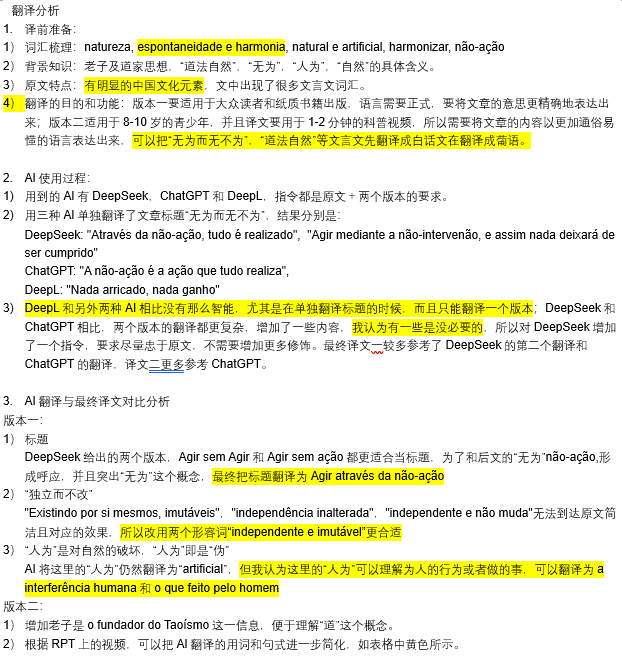
\includegraphics[width=\textwidth]{fig.edu.png}
\caption{Captura de tela de um excerto do relatório de um aprendente de PC24 (grifos do original). No relatório, embora manifeste incerteza quanto à adequação dos resultados da IAG incorporados à versão final de sua tradução, o aprendente reivindica a autoria do texto, justificando ao professor o uso ético e crítico que fez da tecnologia.}
\label{fig:edu}
\source{Autoria própria.}
\end{minipage}
\end{figure}

Um terceiro padrão, particularmente evidente em PC23 e PC24, é o uso substitutivo, caracterizado por fluxos de trabalho iniciados em chinês e mediados, inicialmente, por sistemas de tradução automática (como DeepL ou Google Tradutor). A IA é acionada apenas numa etapa posterior, para revisão de estilo ou adequação a normas discursivas da língua portuguesa. Segundo os aprendentes, esse processo preserva o controle sobre a “autoria das ideias”: os estudantes mantêm maior controle sobre o conteúdo conceptual e recorrem à IA apenas para refinar a forma, evitando que o algoritmo “pense por eles”. Essa lógica é visível em relatos como o de um aprendente que afirmou preferir traduzir no DeepL e, apenas depois, pedir ajustes ao DeepSeek para “não perder o sentido original”. O fato de esse comportamento aparecer tanto em EP quanto em PC sugere um padrão transversal entre cursos e níveis de proficiência.

As práticas de uso da IA também revelam tensões que atravessam autoria, agência e avaliação. Em entrevista, docentes relataram dificuldade em atribuir autoria a trechos altamente fluentes, especialmente quando, durante as apresentações orais, os estudantes não conseguem justificar suas escolhas. Em algumas produções finais, encontramos estruturas formulaicas típicas de IA: conectores excessivamente neutros, construções universalizantes ou variações estilísticas pouco compatíveis com o repertório linguístico demonstrado pelos estudantes em diferentes situações. Essa dissociação entre proficiência performada e proficiência efetiva foi igualmente observada em \textcite{AmaroPires2024}, os quais mostraram que a IA pode ampliar controle linguístico, mas também reduzir controle sobre ideias, criando tensão entre qualidade aparente e profundidade interpretativa.

Apesar disso, os aprendentes não adotam a IA de forma acrítica. Há indícios claros de resistência seletiva e de curadoria pessoal da agência. Muitos preferem confiar na IA para correção formal, porém rejeitam sua intervenção em processos de ideação ou desenvolvimento argumentativo, como expressou uma aprendente de PC24: “a IA melhora o texto, mas não quero que ela pense por mim”. Esses posicionamentos refletem a recalibração da agência no processo de escrita multilíngue, segundo a qual estudantes ajustam a sequência humano-máquina para preservar autoria conceitual.

Do ponto de vista sociolinguístico, os dados revelam ecologias linguísticas complexas e evidenciam o reconhecimento dos aprendentes sobre o pluricentrismo da língua portuguesa. Embora o português seja a língua-alvo, a discussão de questões linguísticas é majoritariamente conduzida em chinês (mandarim e cantonês), tanto em interações presenciais quanto em ecossistemas digitais (\textit{vide} \Cref{fig:edu}). Na produção escrita, observamos dilemas relacionados às diferentes ortografias e variedades do português (Acordo Ortográfico de 1990, ortografia de 1945, variantes brasileira, europeia e português de Macau), o que leva estudantes a solicitar à IA correções coerentes com a variedade desejada. Dois prompts recorrentes nos relatórios foram “\textchinese{將以下文本從巴葡轉換為葡葡}[converta português brasileiro para português de Portugal]” e “\textchinese{將以下文本從簡體轉換為繁體中文}[converta chinês simplificado para chinês tradicional] \footnote{Em relação à grafia do chinês, Macau adota o sistema de caracteres chineses tradicionais, enquanto a China continental utiliza caracteres chineses simplificados.}, o que aponta que a IA é constantemente utilizada para calibrar ortografia, variedade e registro tanto no português como no chinês. Descrevemos essa dinâmica como “calibração da agência situada”, em que a IA é usada para estabilizar escolhas normativas em contextos superdiversos nos quais convivem múltiplos padrões.

Outro aspecto que emerge das entrevistas é o impacto da chamada “explosão do DeepSeek” e sua rápida popularização na China. Nesse contexto, um aprendente da turma EP24 relatou: “não preciso mais de VPN [rede privada virtual] e também me sinto mais confiante em usar uma IA pensada para os chineses [...] DeepSeek dá respostas mais naturais quando eu pergunto em chinês”. Professores entrevistados corroboram esse fenômeno apontando que o DeepSeek “catapultou” e “normalizou” o uso da IA entre os estudantes, tornando-se parte integrante das rotinas de escrita, revisão e consulta de dúvidas – especialmente entre os aprendentes que ingressaram na licenciatura em PLE a partir de 2024.

Há, contudo, diferenças entre os cursos analisados. Em EP, nota-se forte dependência da tradução como ponto de partida, especialmente entre estudantes que se sentem inseguros para elaborar diretamente em português. A IA é utilizada para formatar, ajustar registro e corrigir ortografia, com marcas de correção automatizada mais frequentes em textos curtos e formais. Em PC, a IA é frequentemente acionada para verificação de referências, conversão de estilos, revisão ortográfica e síntese de literatura. Estudantes tendem a verificar se a IA “compreendeu” corretamente um texto antes de solicitar resumos ou traduções, procedimento observado em tarefas de resumos acadêmicos e revisões de literatura documentadas no nosso \textit{corpus}.

Em síntese, os resultados mostram que o uso da IA está profundamente entranhado nas práticas de escrita e tradução nas salas de aula de PLE em Macau, seguindo sequências humanas-máquina relativamente estáveis (ideação $\rightarrow$ escrita em L1 $\rightarrow$ tradução automática $\rightarrow$ polimento por IAG). Produções discentes apresentam autorias híbridas e interdependências entre línguas, com o chinês sustentando processos de negociação oral e o português consolidando-se na escrita. Ao mesmo tempo, persistem tensões ético-pedagógicas relativas à autoria, avaliação, normatividade linguística e formação docente. Esses achados servem de base empírica para a análise conceitual desenvolvida seção seguinte.


\subsection{Análise}\label{sec-ana}

\subsubsection{Dimensão político-institucional}\label{sec-ana-dim}

No que se refere a regulamentos ou diretrizes sobre o uso de IA no ensino superior de Macau, realizamos consultas em português, chinês e inglês aos websites das instituições de ensino superior que oferecem licenciaturas em língua portuguesa, bem como aos portais dos órgãos públicos responsáveis pela organização e gestão da educação no território. Para essa investigação, utilizamos as 24 variações do termo “inteligência artificial” listadas no \textit{Library of Congress Subject Headings}\footnote{Disponível em: \url{https://www.loc.gov/aba/publications/FreeLCSH/freelcsh.html}. Acesso em: 18/9/2025.} . Entre julho e dezembro de 2025, localizamos 18 materiais relacionados ao uso da IA na educação, sendo 13 notícias publicadas nos portais do governo de Macau e 5 orientações gerais emitidas por universidades. No entanto, nenhum desses documentos apresenta menções explícitas a regras específicas de uso. Nesse \textit{corpus}, identificamos 3 lacunas principais: (i) a ausência de critérios explícitos que delimitem usos aceitáveis e não aceitáveis da IA na produção de tarefas e/ou avaliações de ensino; (ii) a inexistência de diretrizes para a atribuição de autoria ou para a aplicação de penalidades em casos de má conduta acadêmica relacionada ao uso de IA; e (iii) a omissão de referências ao multilinguismo e às especificidades do ensino de línguas estrangeiras na regulação institucional dessas práticas.

A ausência de diretrizes específicas faz com que estudantes e docentes operem em um regime de autorregulação, no qual decisões críticas são tomadas localmente, sem amparo normativo. Esse cenário confirma a presença dos \textit{discursos de resposta imperativa} descritos por \textcite{BearmanRyanAjjawi2023}: a IA é tratada institucionalmente como símbolo de modernização e alinhamento internacional, mas sem equivalente investimento em políticas que considerem suas implicações socioculturais, linguísticas e pedagógicas. 

Essa assimetria é particularmente significativa em um território cuja ecologia sociolinguística combina português e chinês nas esferas institucionais e pelo uso do cantonês, do mandarim, do inglês e de outras línguas do sudeste asiático nas esferas cotidianas. As produções discentes evidenciam repertórios híbridos e alternância entre L1, tradução automática e IAG, coerentes com essa pluralidade. No entanto, nos documentos institucionais analisados, não localizamos reconhecimento das implicações do uso da IA para a preservação dessa pluralidade nem problematizações de como tecnologias treinadas majoritariamente em \textit{corpora} anglófonos podem reforçar hierarquias linguísticas. Desse modo, políticas que deveriam orientar a preservação da ecologia linguística acabam por invisibilizar os próprios repertórios que estruturam a aprendizagem em Macau.

Assim, a dimensão político-institucional, além de revelar lacunas regulatórias, aponta um descompasso entre a velocidade da adoção tecnológica e a elaboração de políticas sensíveis ao multilinguismo. A integração da IA no ensino de línguas não se limita a decisões técnicas; ela envolve disputas sobre legitimidade linguística, agência docente e responsabilidade epistêmica, moldando diretamente as tensões observadas nas dimensões pedagógica e ético-humanista.


\subsubsection{Dimensão pedagógica}\label{sec-ana-ped}

Os padrões de uso identificados na \cref{sec-ana-dim} – assistivo, orientado e substitutivo – configuram uma ecologia de aprendizagem na qual inteligências humanas e artificiais se coproduzem. O modo assistivo, exemplificado pelo uso de IA para microcorreções, indica tanto ampliação da autonomia lexical e morfossintática quanto deslocamento da prática reflexiva tradicional para interações de baixa carga cognitiva mediadas por algoritmos. O modo orientado, no qual a IA participa como coautora estilística, intensifica a fluência textual, mas tende a suavizar marcas de autoria individual, produzindo textos altamente polidos, porém homogêneos. Quanto ao modo substitutivo, caracterizado por fluxos iniciados em chinês e mediados por tradução automática, evidencia uma estratégia deliberada para preservar a autoria das ideias enquanto se delegam etapas formais à IA.

Esses padrões sugerem que estudantes calibram sua agência ao longo do processo de escrita, preservando controle conceitual ao mesmo tempo que recorrem à IA para estabilizar escolhas normativas ou elevar a redação final. Entretanto, essa ecologia híbrida produz tensões: a fluência aprimorada não se traduz necessariamente em maior consciência metalinguística, como demonstrado pelas dificuldades em justificar decisões linguísticas durante avaliações orais. Em outras palavras, a IA tende a ampliar a superfície textual, mas não necessariamente o entendimento estrutural do sistema linguístico.

Do ponto de vista docente, esse cenário reconfigura profundamente as práticas pedagógicas. As entrevistas mostram sentimentos de ambivalência: reconhecimento de que a IA apoia a produção escrita, mas também receio quanto à perda de visibilidade do processo e à dificuldade em avaliar autoria. Esses desafios são coerentes com estudos recentes que enfatizam a necessidade de literacias éticas e emocionais na formação docente \cite{SperlingEtAl2024, XieEtAl2025}. A presença constante de IA exige tarefas que provoquem reflexão, comparação entre versões, explicitação de critérios e justificativas metacognitivas, ou seja, um deslocamento da prática avaliativa de produtos para processos.

Diante desses elementos, o papel do professor se transforma: deixa de ser transmissor exclusivo de conhecimento para atuar como curador crítico das práticas mediadas por IA, responsável por promover conhecimento em sua dimensão \textit{phronesis} – discernimento, criatividade, ética e autonomia interpretativa aliados aos conhecimentos teóricos (\textit{episteme}) e práticos (\textit{techne}). Essa transformação reforça o vínculo entre práticas pedagógicas, agência distribuída e condições socioculturais específicas do ensino multilíngue em Macau.


\subsubsection{Dimensão ético-humanista}\label{sec-ana-et}

A dimensão ético-humanista aprofunda questões observadas empiricamente e evidencia implicações que ultrapassam preocupações técnicas. A opacidade das IAG, a fragilidade das fronteiras de autoria e a tendência de algoritmos treinados em \textit{corpora} anglófonos a reproduzirem padrões hegemônicos constituem riscos reais para a construção de conhecimento linguístico em contextos plurilíngues. Nos dados analisados, esses riscos se tornam visíveis na padronização discursiva de textos, na diminuição da diversidade estilística e na supressão de marcas de identidade linguística dos estudantes. Esses aspectos dialogam com a crítica de \textcite{Agnihotri2025} sobre a necessidade de compreender a multilingualidade como condição epistêmica, e não apenas sociolinguística.

A \textit{literacia} \textit{crítica} \textit{em IA} oferece um enquadramento particularmente útil para interpretar esses desafios. Ser letrado criticamente em IA implica ser capaz de questionar vieses, identificar limitações semânticas, interpretar \textit{outputs} de modo contextualizado e reconhecer os contornos éticos que moldam relações entre linguagem, cultura e tecnologia. A análise das práticas docentes e discentes mostra que essas competências ainda não estão institucionalizadas, emergindo de forma fragmentada e dependente da iniciativa individual. Isso reforça a necessidade de articular pedagogias que superem o tecnicismo e promovam a reflexão crítica sobre a IA como fenômeno sociocultural.

Essa reflexão converge com a educação humanista digital \cite{AmaroZhang2025, PiresAmaro2025}, que propõe uma ética da interdependência entre inteligências humanas e artificiais. Em tal perspectiva, formar professores para trabalhar com IA não significa apenas capacitá-los tecnicamente, mas prepará-los para exercer uma “pedagogia do discernimento”, capaz de situar a tecnologia em práticas epistêmicas responsáveis, culturalmente sensíveis e orientadas pela justiça linguística.

\section{Discussão e conclusões}\label{sec-conclusao}

A análise desenvolvida neste artigo sugere que, nos contextos investigados, a integração da IA ao ensino de PLE em Macau reconfigura práticas de escrita, avaliação e mediação docente. Trata-se de reconfiguração epistemológica, pedagógica e ética do modo como se ensina, se aprende e se pensa a linguagem em ecologias híbridas de interação. Os dados empíricos mostram que estudantes e professores atuam em espaços de convergência e fricção, as \textit{interligências} propostas por \textcite{PiresAmaro2025}, nos quais inteligências humanas e artificiais se coproduzem, redistribuindo agência e remodelando práticas de escrita, tradução e avaliação. Essa coprodução não é neutra, pois repercute na formação de identidades linguísticas, nos modos de participação discursiva e na própria concepção de autoria.

No plano político-institucional, os documentos analisados associam a inovação tecnológica a metas de modernização e eficiência, mas não oferecem orientações específicas sobre o uso da IA na promoção do multilinguismo e da diversidade linguística, bem como a sua integração nos currículos e na formação docente. Numa perspectiva pluricêntrica, essa lacuna afeta diretamente o ensino do PLE em Macau, pois os resultados apontam que os aprendentes rotineiramente precisam negociar e justificar escolhas sobre variedade e registro. Do ponto de vista pedagógico, os dados indicam que a IA pode ampliar o repertório linguístico na escrita e apoiar a personalização da revisão, mas não garante, por si só, maior consciência metalinguística. Os estudantes utilizam sequências estáveis de interação, como ideação em L1, \textit{workflows} baseados em tradução automática e polimento por IAG, o que eleva a qualidade formal dos textos sem necessariamente fortalecer o raciocínio linguístico. Docentes entrevistados no \textit{corpus} reconhecem ganhos na revisão e no \textit{feedback}, mas relatam dificuldade em atribuir autoria e em desenhar tarefas que preservem a agência humana. Essas tensões, observadas no corpus deste estudo, ilustram o paradoxo central da educação linguística na era da IA: quanto mais eficiente o sistema, maior a possibilidade de empobrecimento da reflexão sobre a linguagem.

Esse cenário exige redefinição do papel docente. O professor deixa de ser transmissor exclusivo do conhecimento e passa a atuar como mediador ético, curador discursivo e intérprete crítico das interações entre estudantes e algoritmos. A docência contemporânea demanda competências de \textit{literacia em IA} e \textit{literacia e letramento crítico em IA}, além de sensibilidade intercultural e atenção à diversidade linguística. Práticas que comparem traduções humanas e automáticas, analisem apagamentos culturais e explicitem vieses se revelam particularmente eficazes, pois favorecem o desenvolvimento de consciência crítica e engajamento estudantil. A partir dessas práticas, consolida-se a \textit{pedagogia interligente}: um conjunto de práticas didáticas que organiza a colaboração entre inteligências humana e artificial de modo a preservar a agência autoral, explicitar critérios de uso e promover consciência metalinguística e intercultural. Essa pedagogia estimula o estudante a pensar com a IA, sem reproduzir o modo de funcionamento desta, e a tratar o algoritmo como provocação epistêmica, e não como autoridade final.

No plano ético-humanista, os dados reforçam que a IA não ameaça o humano, ela convoca sua reconfiguração. As preocupações com autoria, dependência e autenticidade mostram que a IA funciona como espelho cognitivo que devolve à docência sua dimensão relacional e interpretativa. Nesse contexto, a automatização só adquire sentido quando integrada a um projeto de reumanização do conhecimento \cite{PiresAmaro2025}. Assim, o ensino de línguas torna-se um espaço de coevolução no qual tanto a técnica e a ética se entrelaçam quanto o algoritmo se submete à pluralidade cultural e à responsabilidade educativa.

Considerando nossos resultados, três recomendações orientam o desenvolvimento de políticas e práticas futuras. Primeiro, a formação docente deve integrar dimensões técnicas, éticas e emocionais da literacia em IA, com base em análise de casos reais e práticas reflexivas. Segundo, a avaliação precisa valorizar processos, por meio de atividades que envolvam oralidade, comparação entre versões e justificativas metacognitivas. Terceiro, é necessário fortalecer a governança meso-institucional, articulando políticas linguísticas, ética digital e práticas pedagógicas para reduzir a distância entre uso espontâneo da IA pelos estudantes e sua integração curricular pelas instituições.

Essas recomendações convergem para um princípio geral: a sustentabilidade humanista da inovação digital. O progresso educacional não deve ser medido pela eficiência dos algoritmos, mas pela capacidade de preservar o humano como centro de sentido. A multilingualidade proposta por \textcite{Agnihotri2025} reforça esse princípio ao compreender a linguagem como prática plural, situada e relacional, deslocando o foco da eficiência algorítmica para a justiça linguística e para a agência dos aprendentes. A verdadeira inovação educativa não consiste em ensinar com a IA, mas em ensinar com humanidade em tempos de IA, equilibrando técnica e ética, eficiência e empatia.

Em termos epistemológicos, os resultados reforçam a necessidade de uma educação linguística plural, ética e tecnologicamente crítica. A IA torna visível a coexistência de inteligências múltiplas – humanas, computacionais e institucionais – que operam em um mesmo espaço discursivo. A política linguística, nesse cenário, precisa atuar como ponte entre inovação e equidade, assegurando que a digitalização não se traduza em exclusão, mas em oportunidade de diálogo intercultural.

Este estudo apresenta limites que precisam ser explicitados. Trata-se de um recorte qualitativo e situado em um contexto específico do ensino superior em Macau, com 67 estudantes e mediação de um mesmo docente. Por isso, seus resultados não objetivaram generalização estatística, mas interpretação contextualizada de práticas de escrita, avaliação e uso de IA. Pesquisas futuras poderão ampliar o corpus documental e docente, comparar outros contextos de PLE e acompanhar longitudinalmente os efeitos da IA sobre autoria, revisão e formação docente.

Em síntese, no recorte analisado, humanização e automatização aparecem menos como polos excludentes do que como dimensões em tensão e complementaridade. O conceito de \textit{interligências} oferece uma chave interpretativa para compreender esse equilíbrio dinâmico e permite vislumbrar uma formação docente capaz de atuar nas fronteiras das inteligências com discernimento, sensibilidade intercultural e compromisso com o humano. Nesse horizonte, a IA não é ameaça nem substituto, ela é parceira epistêmica que amplia as capacidades humanas e, ao mesmo tempo, leva-nos a reconhecer a fragilidade e a potência que constituem a experiência de aprender e ensinar línguas.



\printbibliography\label{sec-bib}
% if the text is not in Portuguese, it might be necessary to use the code below instead to print the correct ABNT abbreviations [s.n.], [s.l.]
%\begin{portuguese}
%\printbibliography[title={Bibliography}]
%\end{portuguese}


\begin{dataavailability}
\txtdataavailability{dataonly} % options: dataavailable, dataonly, databody, datanotav, nodata
\end{dataavailability}


%\appendix 


\end{document}

